\documentclass[12pt, a4paper]{article}
\usepackage{graphicx}
\usepackage[slovenian]{babel}
\usepackage{csquotes}
\usepackage{biblatex}
\usepackage{amsmath}
\usepackage{float}
\addbibresource{porocilo.bib}
\graphicspath{{images/}}
\title{Zharko - upodabljanje s sledenjem žarkov}
\author{Filip Trplan}
\date{Avgust 2025}

\begin{document}
\maketitle

\begin{figure}[h]
	\centering
	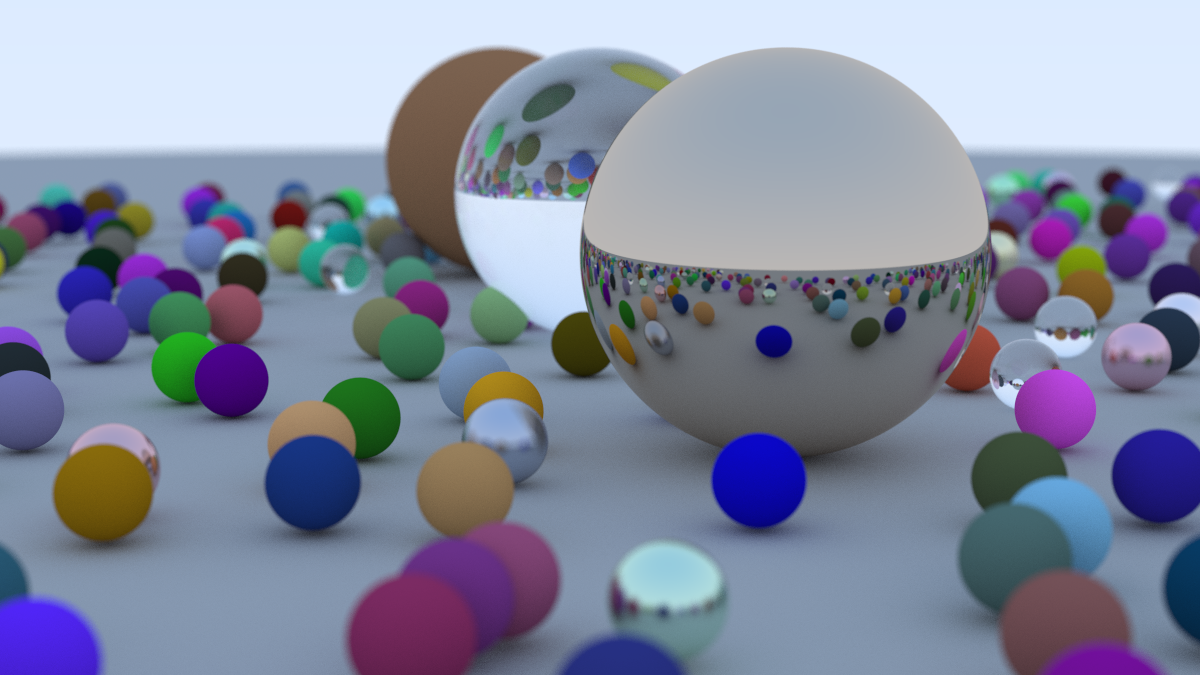
\includegraphics[width=\textwidth]{cover}
	\caption{Koncni rezultat}
\end{figure}

V temu porocilu bom predstavil tehniko upodabljaljanja (\textit{rendering}) s sledenjem zarkov
(\textit{ray tracing}). Lotil se bom prvo osnov sledenja zarkov in bom nato presel na ustvarjanje treh
razlicnih tipov materialov ter koncal z simulacijo globinske ostrine (\textit{depth of field}).

Vseskozi porocila se zgledujem po knjigi \textit{Ray Tracing in One Weekend} \cite{Shirley2025RTW1}

\section{Osnove sledenja zarkov}

Osnovna ideja upodabljanja s sledenjem zarkov je, da si predstavljamo prikazano sliko kot ploskev in kamero
orientirano v 3D prostoru. V realnem svetu svetloba izvira iz svetlobnih virov kot so sonce ali luci in se
nato odbije od raznih objektov dokler ne doseze nasega ocesa oz. senzorja na kameri. Ker pa veliko teh zarkov
zgresi naso kamero, bomo obrnili smer zarkov in jih bomo izstrelili iz kamere.

Zarek bo potoval iz kamere skozi piksel nasem vidnem oknu (\textit{viewport}) ter se nato odbil po
virtualnem svetu dokler ne bo dosegel svetlobnega vira (v nasem primeru bo to nebo).

\begin{figure}[H]
	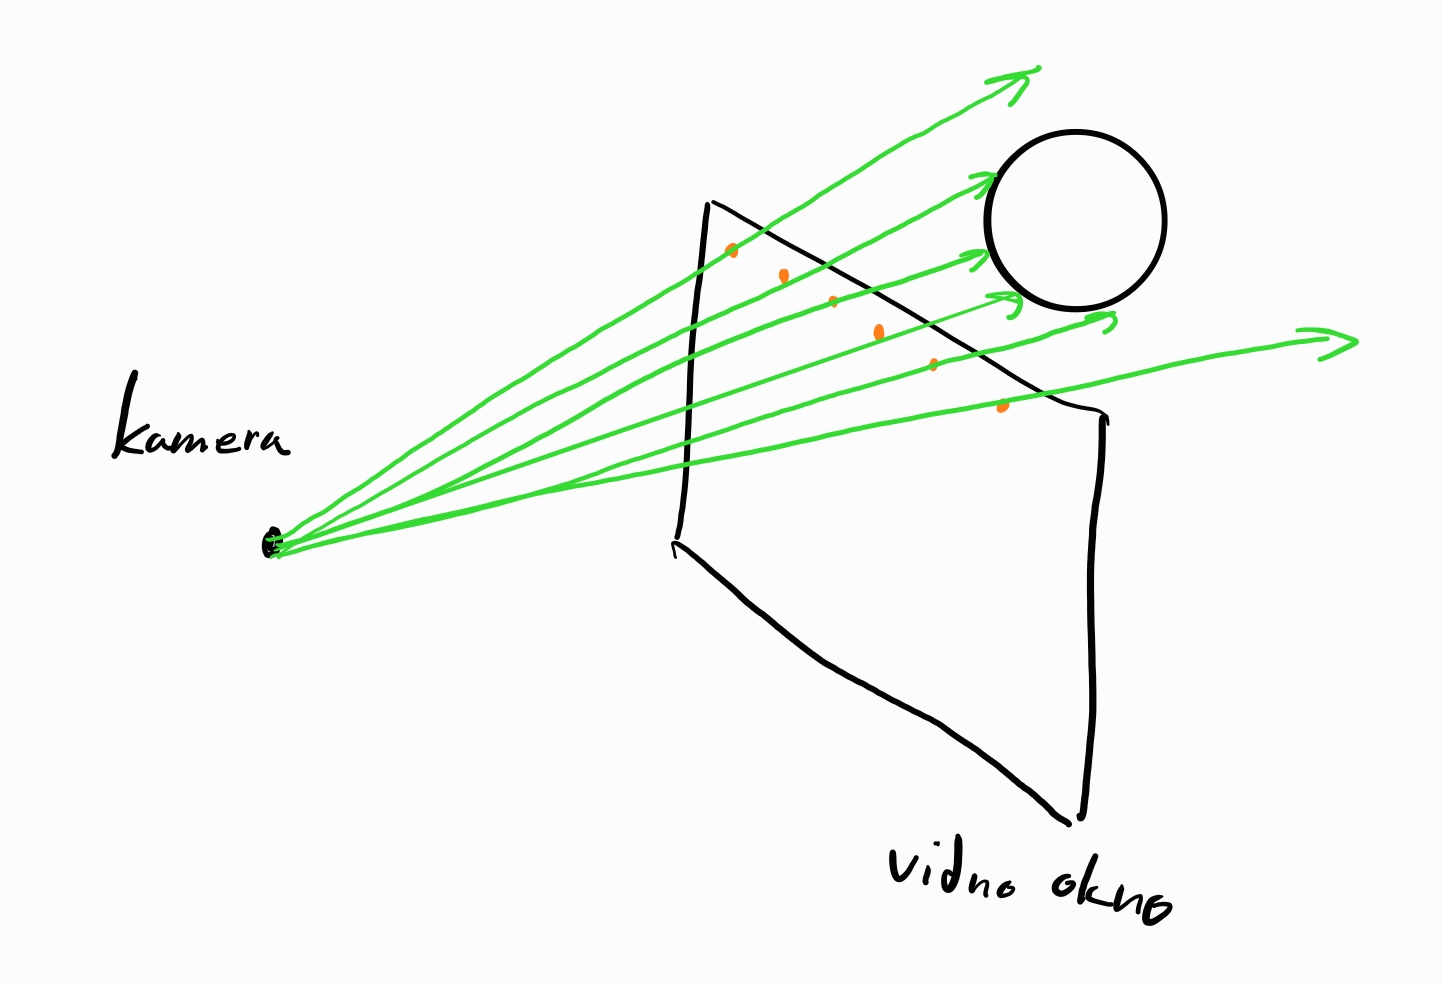
\includegraphics[width=\textwidth]{shema_zarki}
	\caption{Shema sledenja zarkov}
\end{figure}

Vpeljimo par oznak, da si bomo lazje predstavljali kako te zarki potekajo. Pozicijo kamere bomo imenovali $C$,
levi zgornji piksel bo $P_{00}$ in ce so piksli na mrezi, bodo enakomerno razporejeni tako da bo v horizontalni
smeri jih locil vektor $\Delta u$ in v vertikalni $\Delta v$. Prikazane so na sliki \ref{fig:oznake}.

\begin{figure}[h]
	\centering
	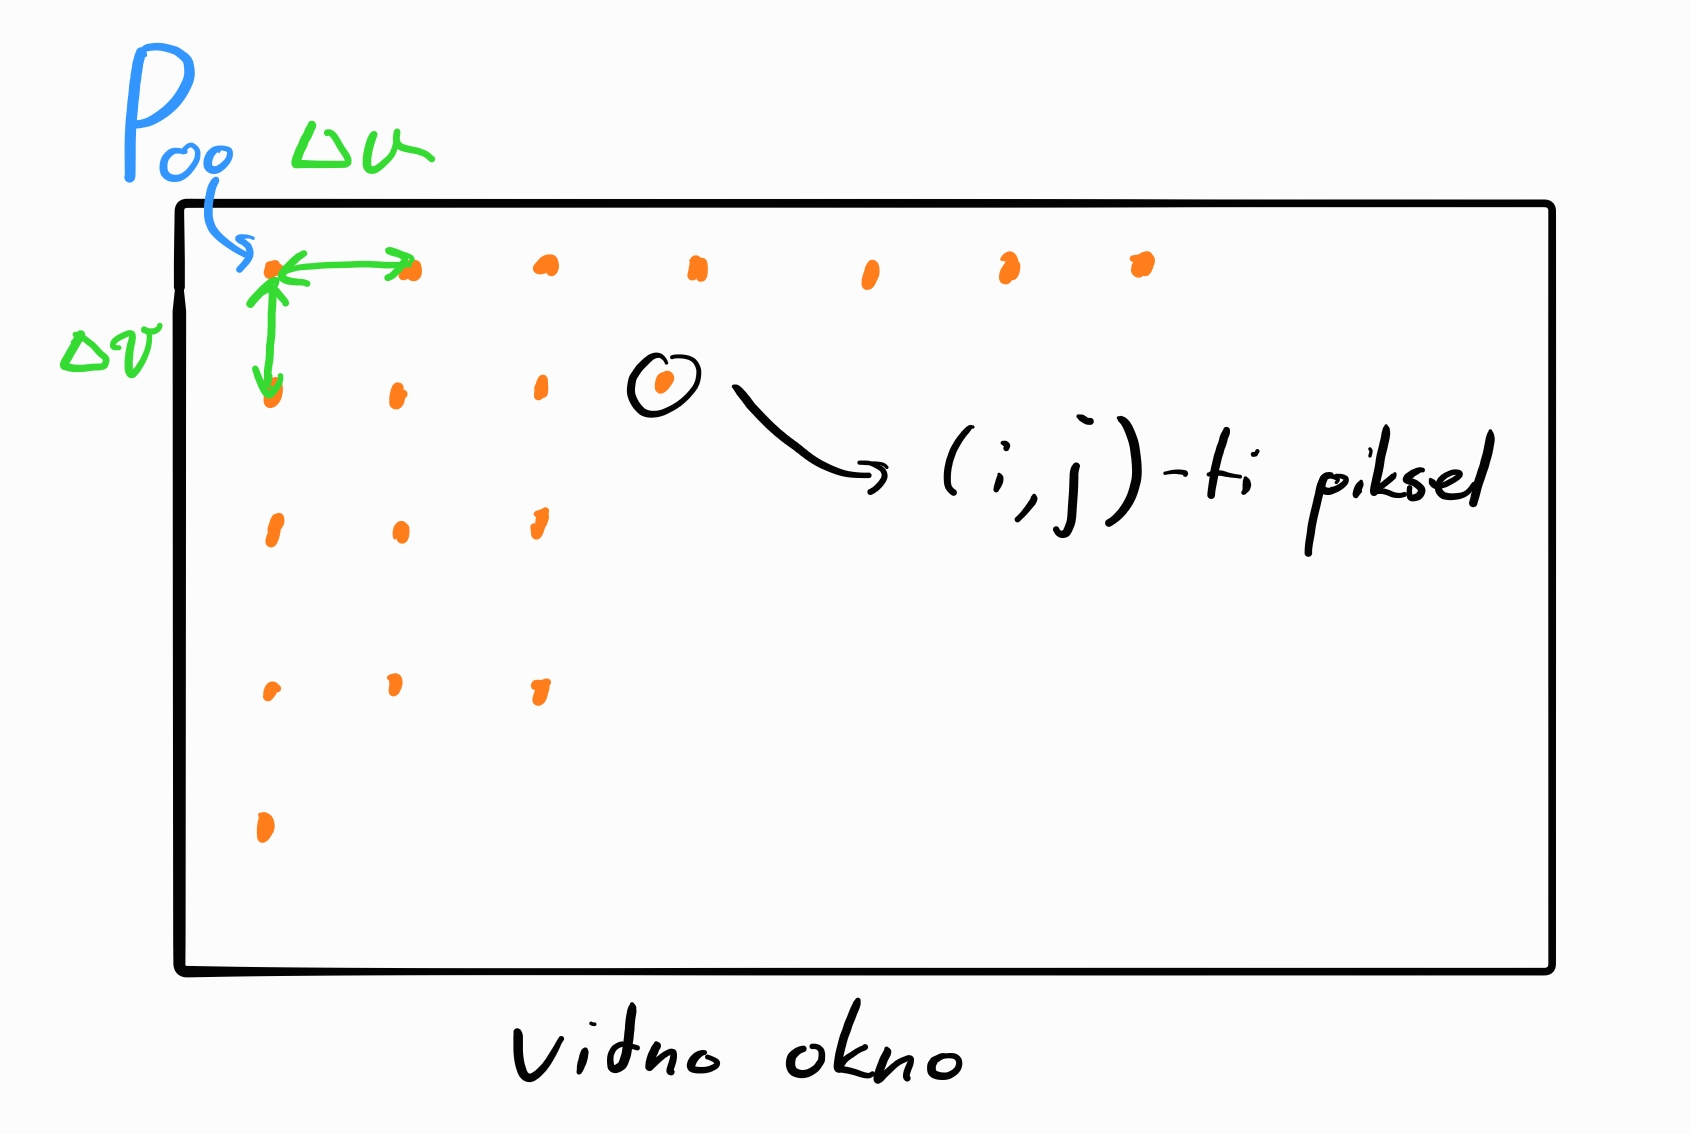
\includegraphics[width=\textwidth]{vidno_okno}
	\caption{Oznake prikazane vizualno}
	\label{fig:oznake}
\end{figure}

Potem lahko zarek $\vec{r}$, ki potuje skozi piksel $(i,j)$ parametriziramo s $t$:

\begin{equation}
	\vec{r} = C + t \cdot (P_{00} + i \cdot \Delta u + j \cdot \Delta v - C)
\end{equation}

V prihodnje pa bomo obravnavali splosne zarke z izvorom v $O$ in smerjo $\vec{d}$.

\section{Detekcija trka}

Trenutno nasi zarki samo streljajo v praznino zato bomo zdaj v svet dodali objekte v katere lahko zarki trcijo.
Matematicno je najlazje opisati sfero. Splosna enacba za sfero s srediscem $C$ in radijem $r$ je

\begin{equation}
	\label{eq:sfera}
	(C_{x} - x)^2  + (C_{y} - y)^2  + (C_{z} - z)^2  = r^2
\end{equation}

Ce tocko $(x,y,z)$ oznacimo kot $P$ lahko \ref{eq:sfera} zapisemo kot skalarni produkt.

\begin{equation}
	(C - P)(C - P) = r^2
\end{equation}

Nasa tocka pa lezi na zarku torej dobimo

\begin{equation}
	(C - (O + t \vec{d}))(C - (O + t \vec{d})) = r^2
\end{equation}

Po nekaj preurejanja enacbe dobimo naslednjo kvadratno enacbo

\begin{equation}
	t^2 \lVert C \rVert ^2  - 2 t \cdot \vec{d} (C - O) + \lVert C - O \rVert ^2  - r^2 = 0
\end{equation}

S pomocjo diskriminante lahko zlahka preverimo ali nas zarek sploh zadane sfero. Ce resitev obstaja pa vzamemo
najmanjso pozitivno (torej najblizjo kameri v smeri pogleda). V primeru, da pozitivna resitev ne obstaja pa
smatramo, kot da zarek ni zadel objekta, saj je za kamero.

Na sliki \ref{fig:red_sphere} vidimo primer izrisa sfere, kjer jo samo obarvamo samo z rdeco barvo.

\begin{figure}[H]
	\label{fig:red_sphere}
	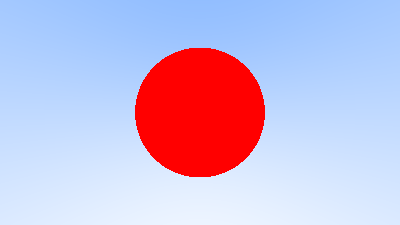
\includegraphics[width=\textwidth]{red_sphere}
	\caption{Rdece obarvana sfera}
\end{figure}

Na zgornji sliki vidimo, da ima sfera zagast rob. To se zgodi zaradi diskretizacije pikslov v mrezo. Temu
pojavimo pravimo \textit{aliasing}. Znebimo se ga tako, da za vsak piksel izstrelimo vec zarkov ki so nakljucno
pertrubirani za najvec polovicno razdaljo med piksli, ter nato barvo teh zarkov povprecimo. Tehnika se imenuje
MSAA (\textit{multisample anti-aliasing}) in smo jo izbrali, ker je v kontekstu sledenja zarkov najbolj
enostavna za implementirati.

\section{Materiali}

\subsection{Difuzni materiali in Lambertov odboj}

Prve materiali, ki se jih bomo lotili so difuzni. Taki materiali v realnem svetu zgledajo mat in so takega
videza, ker se zarki nakljucno odbijejo od povrsine objekta. Lambertov odboj je aproksimacija takih materialov,
ki pravi, da naj je smer odbitega zarka izbrana sorazmerno s kolicino $\cos (\phi) $, kjer je $\phi$ vpadni
kot.

\begin{figure}[H]
	\centering
	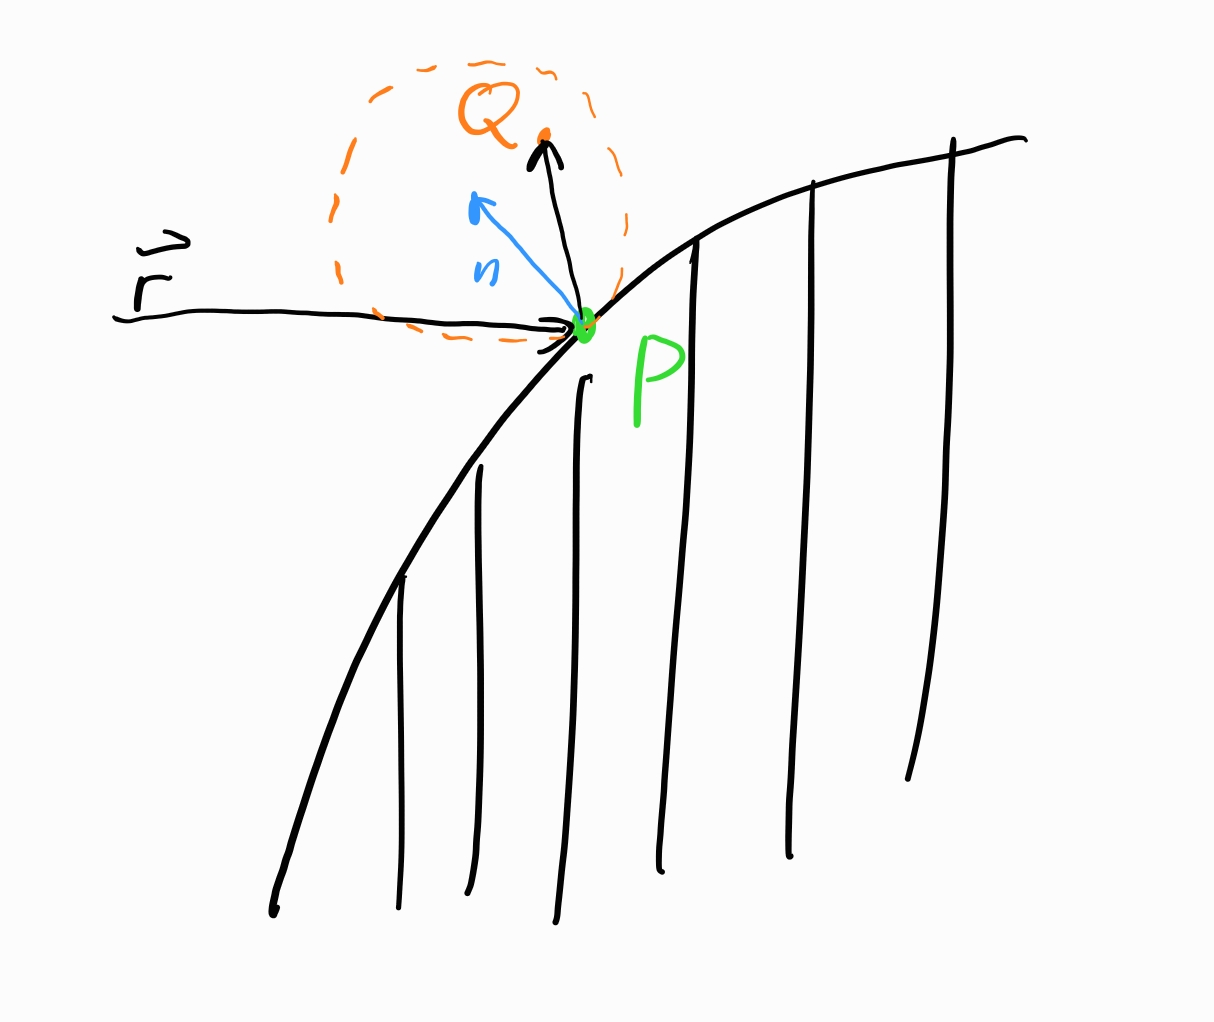
\includegraphics[height=250pt]{shema_difzuni}
	\caption{Lambertov odboj}
\end{figure}

Ce zarek seka objekt na tocki $P$ in je normala povrsine vektor $n$, potem izberemo nakljucno tocko $Q$
znotraj enotske sfere s srediscem $P + n$ (kjer je normala enotski vektor). Smer odbitega zarka je potem
$Q - P$.

\begin{figure}[H]
	\centering
	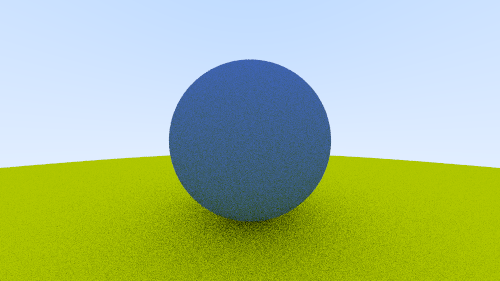
\includegraphics[width=400pt]{difuzni}
	\caption{Dve difuzni sferi}
\end{figure}

Da dodamo barvo, odbiti žarek pomnožimo z barvo objekta, ki ji pravimo \textit{albedo}. Tako se barva
svetlobnega vira postopoma spreminja ob vsakem odboju - množi se z albedo vsakega objekta, s katerim se
žarek sreča. Končna barva piksla je zato produkt barve svetlobnega vira in vseh albedo vrednosti
objektov na poti žarka.

\textit{Opomba: }, ker se ta metoda zanasa na nakljucne procese za aproksimacijo realnega sveta (Monte Carlo),
dobimo nekaj suma v sliki.

\subsection{Kovinski materiali}

Kovine imajo svojo barvo, vendar pa hkrati tudi odbijejo del svetlobe pod istim kotom, kot je
zarek srecal objekt. Odbiti zarek je sestavljen iz dveh delov: zrcaljeni del in t.i. zamegljeni del
(\textit{fuzziness}). Koncni odbiti zarek je vsota teh dveh vektorjev.

\begin{figure}[H]
	\centering
	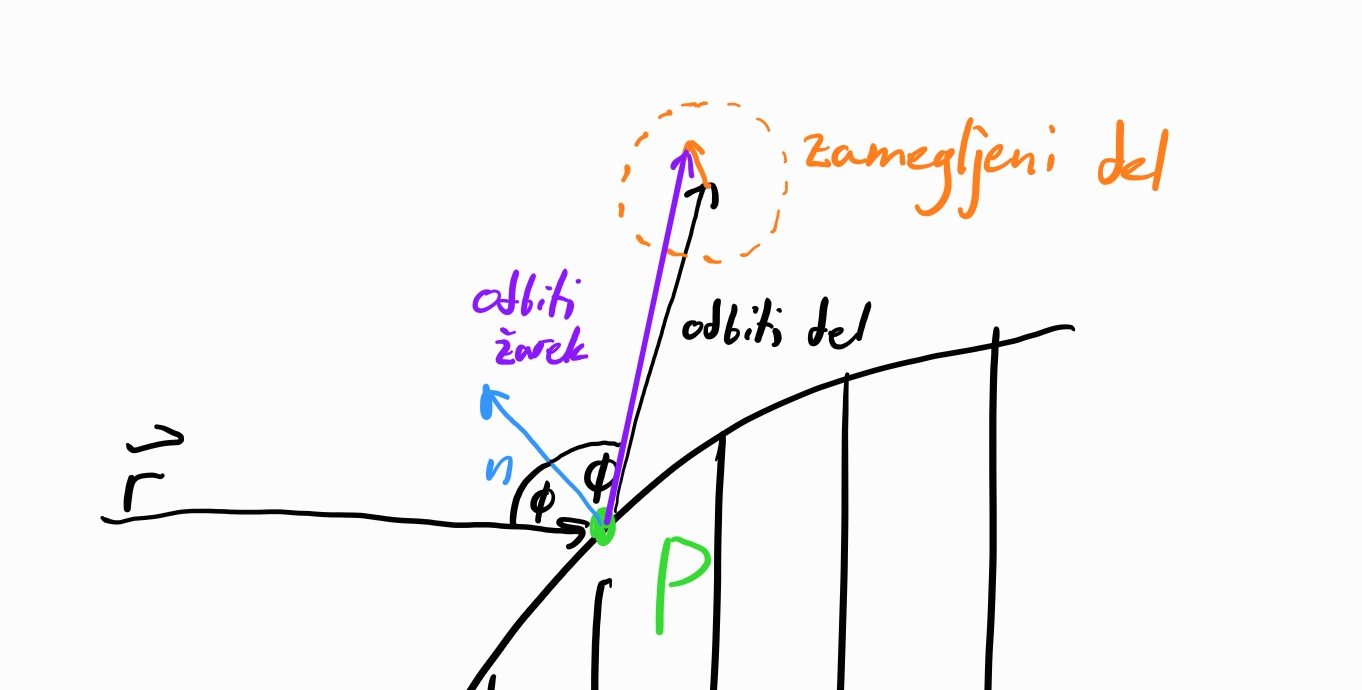
\includegraphics[width=400pt]{metal}
	\caption{Odboj zarka od kovinskega materiala}
\end{figure}

Zrcaljeni del je preprosto vpadni zarek zrcaljen cez ploskev, ki jo opise normala in z zamenjano smerjo.
Zameglejni del pa simulira hrapavost kovine in je samo nakljucni vektor znotraj enotske sfere pomnozen
s parametrom $0 \leq f \leq 1$, ki kontrolira kako zamegljen je objekt.

\subsection{Dielektricni materiali}
Še zadnja vrsta materialov, ki jih uporabljamo, so prosojni materiali oziroma dielektriki. To so na primer voda,
steklo in diamant. Ko svetloba preide skozi te materiale se upogne, ko prehaja med dvema materialoma z
različnima lomnima kolicnikoma. Na primer, zrak ima kolicnik blizu 1, steklo pa okoli 1,5. Lom svetlobe opisujemo
z lomnim zakonom.

$$
	tukaj zakon
$$

% tukaj bom dal se diagram zakona

Lomni zakon ni vedno rešljiv — pri prevelikem vpadnem kotu nastopi popolni notranji odboj — svetloba se v takem
primeru v celoti odbije od meje med materialoma, namesto da bi prešla v drugi medij. Tudi ce je enacba resljiva
pa se svetloba ne lomi v celoti, nek delez se vedno odbije od materiala. Ta pojav opisujejo Fresnelove enacbe, ki
so odvisne od vpadnega kota. Ker pa je resevanje tega sistema pocasno, v praksi uporabimo polinomsko Schlickovo
aproksimacijo

$$
	schlickova aproksimacija
$$

Torej v praksi bomo uporabljali Monte Carlo metodo, kjer se zarek odbije od povrsine materiala, ce lomni zakon
ni resljiv ali pa velja $nakljucno stevilo < Schlickova aproksimacija$.

\section{Globinska ostrina}

V pravi kameri je leča sestavljena iz več steklenih elementov, ki so za odprtino, ki ji pravimo zaslonka.
Zaradi tega, ker je ta odprtina vecja od tocke, bodo objekti na doloceni razdalje povsem ostri, ostali pa
zamegljeni. Temu pojavu pravimo globinska ostrina. Namesto modeliranja kompleksnega sistema vecih elementov
pa bomo uporabili model tanke lece.

% skica tanke lece in zakaj zarki niso ostri

Efekt bomo simulirali tako, da se bomo pretvarjali, da je pozicija nase kamere v resnici pozicija lece in
da je polozaj nasega vidnega okna ravnina, kjer bodo objekti izostreni.

Kako to dosežemo? Izhodišča žarkov naključno zamaknemo za vektor, izbran v enotskem krogu, in ga skaliramo s
faktorjem, izračunanim glede na odprtost zaslonke. Ti žarki so nato usmerjeni točno v ciljni piksel na vidnem
oknu, vendar zaradi zamaknjenih izhodišč malo odstopajo od pricakovane poti pred in po oknu, kar ustvari učinek
globinske ostrine.

\printbibliography

\end{document}
